\documentclass[a4paper,12pt]{article}

\usepackage{time}
\usepackage{pst-vue3d}
\usepackage{pstricks,pst-node,pst-text,pst-3d,pst-coil, pst-tree}
\usepackage{amsthm}
\usepackage{amsmath,amssymb}
\usepackage{graphicx}
\usepackage{anysize}
\usepackage{epsfig}
\usepackage{url}
\usepackage{tikz}
\usetikzlibrary{positioning,shapes,arrows}


\title{Prototype software development} 
\author{}
\date{Last update: \today~at \now}


%\theoremstyle{definition}
%\newtheorem{definition}{Definition}

%\theoremstyle{theorem}
%\newtheorem{theorem}{Theorem}
%\theoremstyle{example}
%\newtheorem{example}{Example}
%\newtheorem{proposition}{Proposition}

\definecolor{verdoso}{rgb}{0,0.7,0}
\newcommand{\fondoverde}[1]{\multicolumn{1}{>{\columncolor{white}}c}{#1}}
\newcommand{\fondoOliveGreen}[1]{\multicolumn{1}{>{\columncolor{OliveGreen}}c}{#1}}
\newcommand{\fondorojo}[1]{\multicolumn{1}{>{\columncolor{red}}c}{#1}}
\newcommand{\amari}[1]{\multicolumn{1}{>{\columncolor{nodecolor}}r}{#1}}
\newcommand{\w}{\mathbf{w}}
\newcommand{\x}{\mathbf{x}}
\newcommand{\y}{\mathbf{y}}
\newcommand{\z}{\mathbf{z}}
\newcommand{\e}{\mathbf{e}}
\newcommand{\be}{\mathbf{b}}


\newcommand{\A}{\mathbf{A}}
\newcommand{\W}{\mathbf{W}}
\newcommand{\X}{\mathbf{X}}
\newcommand{\Y}{\mathbf{Y}}
\newcommand{\Z}{\mathbf{Z}}
\newcommand{\E}{\mathbf{E}}



\newcommand{\Reals}{I\!\! R}
\newcommand{\ele}{\mathbf{l}}
\newcommand{\nai}{na\"{\i}ve~}
\newcommand{\Nai}{Na\"{\i}ve~}
\newcommand{\peq}{\scriptsize}
\newcommand{\de}{\mathbf{d}}
\newcommand{\Var}{\mathrm{Var}}
\newcommand{\Cov}{\mathrm{Cov}}
\newcommand{\dom}{\mathrm{dom}}
\newcommand{\T}{{\cal T}}
\newcommand{\trans}{^{\mathsf{T}}}
\providecommand{\abs}[1]{\lvert#1\rvert}


\newtheorem{proposition}{Proposition}%[section]
%%%%%% MIS COMANDOS GRAFICOS %%%%%%%%%%%%%%%%%%




%\newgray{lightgris}{0.8}
%\newgray{migris}{0.7}
\newcommand{\nborde}[4]{\rput(#1,#2){\rnode{#4}{{\makebox{\centering \scriptsize #3}}}}}
 
 \newgray{grisclaro}{0.9}
  \newgray{grismuyclaro}{0.95}
 
\definecolor{nodecolor}{RGB}{238,221,130}

\definecolor{orange}{RGB}{255,127,0}


\newcommand{\rnod}[4]{\cnode(#1,#2){#3}{N#1-#2}\rput(#1,#2){\tiny #4}}
%\rnod{coorx}{coory}{rad}{text} % :Crea un nodo (con nombre "Ncoorx-coory") en (coorx,coory) de radio rad
\newcommand{\nod}[3]{\cnode(#1,#2){1}{N#1-#2}\rput(#1,#2){\tiny #3}}
%\nod{coorx}{coory}{text}   % :Crea un nodo (con nombre "Ncoorx-coory") en (coorx,coory) de radio la unidad de longitud
\newcommand{\nnod}[4]{\cnode(#1,#2){1.2}{#4}\rput(#1,#2){\footnotesize #3}}
\newcommand{\nnodtwolines}[4]{\cnode[doubleline=true](#1,#2){1.4}{#4}\rput(#1,#2){\footnotesize #3}}

\newcommand{\nnodgris}[4]{\cnode[fillstyle=solid, fillcolor=grisclaro](#1,#2){1.2}{#4}\rput(#1,#2){\footnotesize #3}}

%\nod{coorx}{coory}{text}   % :Crea un nodo (con nombre "Ncoorx-coory") en (coorx,coory) de radio la unidad de longitud con relleno grisclaro



%\nod{coorx}{coory}{text}   % :Crea un nodo (con nombre "Ncoorx-coory") en (coorx,coory) de radio la unidad de longitud y con su linea con estilo dashed
\newcommand{\nnoddashed}[4]{\cnode[linestyle=dashed, fillcolor=white](#1,#2){1.2}{#4}\rput(#1,#2){%
\footnotesize #3}}

 %\nnod{coorx}{coory}{text}{nom}   % :Crea un nodo (con nombre nom) en (coorx,coory) de radio la unidad de longitud
\newcommand{\anod}[3]{\rput(#1,#2){\circlenode{N#1-#2}{%
\tiny #3}}}
%\anod{coorx}{coory}{tex} %  :Crea un nodo (con nombre "Ncoorx-coory") en (coorx,coory) de radio ajustable al texto

\newcommand{\fle}[4]{\ncline[linecolor=black,linewidth=1pt,angleA=#2,angleB=#4, arrowsize = 3pt 3]{->}{#1}{#3}}


\newcommand{\fledashed}[4]{\ncline[linestyle=dashed,linecolor=black,linewidth=1pt,angleA=#2,angleB=#4, , arrowsize = 3pt 3]{->%
}{#1}{#3}}



%\fle{nod1}{ang1}{nod2}{ang2} % Dibuja una flecha desde el nod1 con salida en \'{a}ngulo ang1 al nod2 con entrada en \'{a}ngulo ang2
\newcommand{\ari}[4]{\ncline[linecolor=black,linewidth=1pt,angleA=#2,angleB=#4]{-%
}{#1}{#3}}
%\ari{nod1}{ang1}{nod2}{ang2} % Dibuja una l\'{\i}nea (arista) desde el nod1 con salida en \'{a}ngulo ang1 al nod2 con entrada en \'{a}ngulo ang2
\newcommand{\fledas}[4]{\ncline[linecolor=black,linestyle=dashed,linewidth=1pt,angleA=#2,angleB=#4]{->%
}{#1}{#3}}
%\fledas{nod1}{ang1}{nod2}{ang2} % Dibuja una flecha dashed desde el nod1 con salida en \'{a}ngulo ang1 al nod2 con entrada en \'{a}ngulo ang2
\newcommand{\aridas}[4]{\ncline[linecolor=black,linestyle=dashed,linewidth=1pt,angleA=#2,angleB=#4]{-%
}{#1}{#3}}
%\aridas{nod1}{ang1}{nod2}{ang2} % Dibuja una l\'{\i}nea dashed desde el nod1 con salida en \'{a}ngulo ang1 al nod2 con entrada en \'{a}ngulo ang2
\newcommand{\aridot}[4]{\ncline[linecolor=black,linestyle=dotted,linewidth=1pt,angleA=#2,angleB=#4]{-%
}{#1}{#3}}
%\aridot{nod1}{ang1}{nod2}{ang2} % Dibuja una l\'{\i}nea de puntos desde el nod1 con salida en \'{a}ngulo ang1 al nod2 con entrada en \'{a}ngulo ang2

\newcommand{\aridasgris}[4]{\ncline[linecolor=grisclaro,linestyle=dashed,linewidth=1pt,angleA=#2,angleB=#4]{-%
}{#1}{#3}}
%\aridotgris{nod1}{ang1}{nod2}{ang2} % Dibuja una l\'{\i}nea discont\'{\i}nua color gris desde el nod1 con salida en \'{a}ngulo ang1 al nod2 con entrada en \'{a}ngulo ang2

\newcommand{\novalnod}[4]{\rput(#1,#2){\ovalnode{#4}{\footnotesize #3}}}
\newcommand{\novalnodtwolines}[4]{\rput(#1,#2){\ovalnode[doubleline=true]{#4}{\footnotesize #3}}}
 %\novalnod{coorx}{coory}{text}{nom}   % :Crea un nodo oval (con nombre nom) en (coorx,coory)

 %\novalnod{coorx}{coory}{text}{nom}{fillstyle}{fillcolor}   
 % :Crea un nodo oval (con nombre nom) en (coorx,coory) y con (fillstyle =solid,...) y (fillcolor)
 

\newcommand{\nfram}[6]{\rput(#1,#2){\rnode{#6}{\psframebox{\parbox[c][#3][c]{#4}{%
 \centering \tiny #5}}}}}
 %\nfram{coorx}{coory}{text}{nom}   % :Crea un nodo-caja (con nombre nom) en (coorx,coory) de
 %altura alt y longitud lon y dentro centra text

\newcommand{\nafram}[4]{\rput(#1,#2){\rnode{#4}{\psframebox[fillcolor=white]{\makebox{\centering \scriptsize #3}}}}}
 %\nafram{coorx}{coory}{text}{nom}   % :Crea un nodo-caja (con nombre nom) en (coorx,coory) de
 %y  dentro centra text

\newcommand{\aritexta}[5]{\ncline[linecolor=black,linewidth=1pt,angleA=#2,angleB=#4]{-%
}{#1}{#3}\naput{\tiny{#5}}}


\newcommand{\aritextb}[5]{\ncline[linecolor=black,linewidth=1pt,angleA=#2,angleB=#4]{-%
}{#1}{#3}\nbput{\tiny{#5}}}


%\newcommand{\novalnodtwolines}[4]{\rput(#1,#2){\ovalnode[doubleline=true]{#4}{\footnotesize #3}}}

%\newcommand{\novalnodtwolines}[4]{\cnode[doubleline=true](#1,#2){1.2}{#4}\rput(#1,#2){\footnotesize #3}}
%\cput[doubleline=true](1,.5){\large $K_1$}



%%%%%%%%%%%%%
%\newcommand{\idr}{\perp\!\!\!\perp}
%\renewcommand{\algorithmcfname}{Algoritmo}


%\theoremstyle{definition}
%\newtheorem{definicion}{Definición}[chapter]
%
%\theoremstyle{example}
%\newtheorem{ejemplo}{Ejemplo}[chapter]
%
%\theoremstyle{theorem}
%\newtheorem{teorema}{Teorema}[chapter]
%
%
%\theoremstyle{proposition}
%\newtheorem{proposicion}{Proposición}[chapter]
%

%\newcommand{\nnod}[4]{\cnode(#1,#2){1}{#4}\rput(#1,#2){\tiny #3}}


%\nod{coorx}{coory}{text}   % :Crea un nodo (con nombre "Ncoorx-coory") en (coorx,coory) de radio la unidad de longitud con relleno grisclaro



\begin{document}
\maketitle
\tableofcontents
\section{Introduction}

This document aims at explaining the design of the skeleton of the AMIDST software 
prototype that will include only the basic structures required to easily plug in, in future 
tasks, new inference and learning algorithms within an streaming data framework.  It is
a very first draft that must be refined and expanded with all the functionality. Classes
in the diagrams include only those attributes and methods that are considered important
for this first version of the design.

The prototype should be as generic as possible in the sense that specific features 
of new algorithms directly fit into the toolbox. For that purpose, a interface-based 
implementation will be addressed. At the same time, inheritance will be used only
when absolutely necessary in order not to overload classes in excess. Apart from this 
generality it is important to keep an eye on our three use cases when designing the 
classes as they give us hints
about the different scenarios to be considered for the prototype. 

The data structures of the prototype will covered the following issues:

\begin{itemize}
\item Model representations for static and dynamic hybrid Bayesian networks.
\item Probability estimators for the different types of distributions contained in the 
models. 
\item Potentials for the model variables.
\item Support for processing data streams for static and dynamic models.
\item Support for scalability.  Not sure if scalability influences the design at this stage? Is it specific of the algorithms for learning and inference that will be plugged in later? 
\end{itemize}

In what follows, we explain the key aspects of the different classes that have 
been grouped by conceptual blocks for the ease of presentation, although they 
have some classes in common where all the diagrams are linked. The diagrams have been built using the free 
software Violet UML Editor (\url{http://alexdp.free.fr/violetumleditor/page.php}).



\section{Model representation}\label{sec:modelRepresentation}

For the sake of efficiency, we propose to represent separately static and dynamic 
models. 

%%%%%%%%%%%%%%%%%%%%%%%%%%%%%%%%%%%%%%%%%%

\subsection{Static Bayesian networks}
\label{subsec:staticBNs}


\begin{figure}[h]

\centering
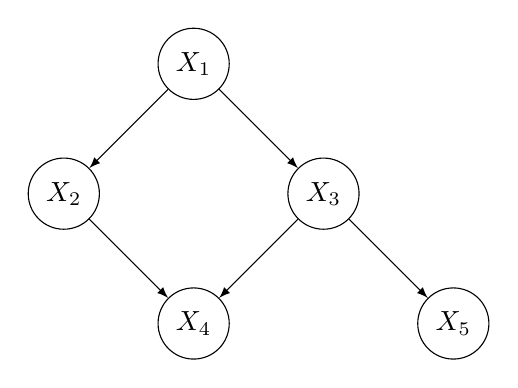
\begin{tikzpicture}[
  node distance=1cm and 1cm,
  mynode/.style={draw,circle,text width=0.5cm,align=center}
]
\node[mynode] (x1) {$X_1$};
\node[mynode,below left=of x1] (x2) {$X_2$};
\node[mynode,below right=of x1] (x3) {$X_3$};
\node[mynode,below right=of x2] (x4) {$X_4$};
\node[mynode,below right=of x3] (x5) {$X_5$};

\path (x1) edge[-latex] (x2)
         (x1) edge[-latex] (x3) 
	(x2) edge[-latex] (x4)
	(x3) edge[-latex] (x4)
	(x3) edge[-latex] (x5)
	;
\end{tikzpicture}
\caption{Static Bayesian network}
\label{fig:staticBN}
\end{figure}





\begin{figure}[h]
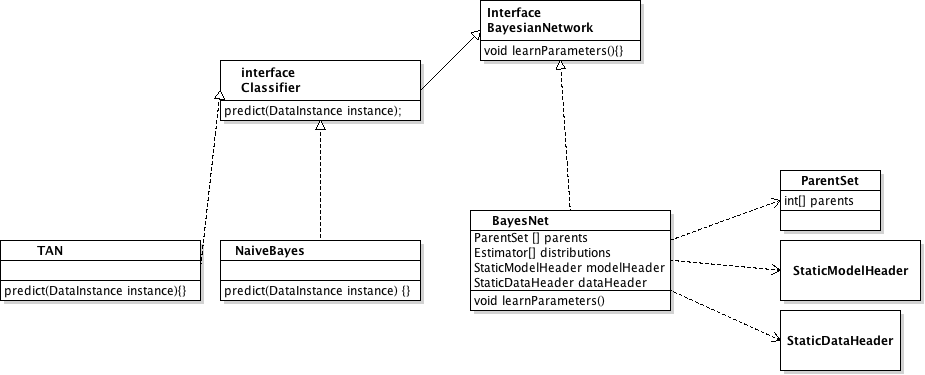
\includegraphics[width=\textwidth]{staticBN}
\caption{Class diagram for the static BNs.}
\label{fig:classDiagramStaticBN}
\end{figure}


The idea is to have an interface called \texttt{BayesianNetwork} for supporting 
different implementations of a static Bayesian network (Fig.~\ref{fig:staticBN}). Our implementation of the 
interface is made through class \texttt{BayesNet}. This class contains several 
attributes:

\begin{itemize}
\item {\bf parents}: a vector of \emph{ParentSet} objects in which each element represent a 
variable in the model. The \emph{ParentSet} object represents the parents as a 
vector of variable IDs. 
\item {\bf distributions}: a vector of \emph{Estimator} objects (see Section~\ref{sec:estimator_potential}), one 
for each variable. 
\item {\bf dataHeader}: a \emph{StaticDataHeader} object (see Section~\ref{subsec:staticDatabase}) with 
the information about the observed variables. 
\item {\bf modelHeader}: A \emph{StaticModelHeader} object (see Section~\ref{subsec:dynamicDatabase}) 
with information about the variables.

\end{itemize}

As classifiers are a BN model with their own behavior, we decided to create their 
own interface called \emph{Classifier} extending from interface 
\emph{BayesianNetwork}. Thus, different classifier models could implement their 
own behavior, e.g., NB, TAN, ...

%%%%%%%%%%%%%%%%%%%%%%%%%%%%%%%%%%%%%%%%%%





\subsection{Dynamic Bayesian networks}
\label{subsec:dynamicBNs}

The idea is to represent a dynamic model with any Markov order $t$. Consider a simple 
static Bayesian network $X \rightarrow Y$. The dynamic version of order $t=2$ 
is shown in Fig.~\ref{fig:dynamicBN}

\begin{figure}[h]

\centering
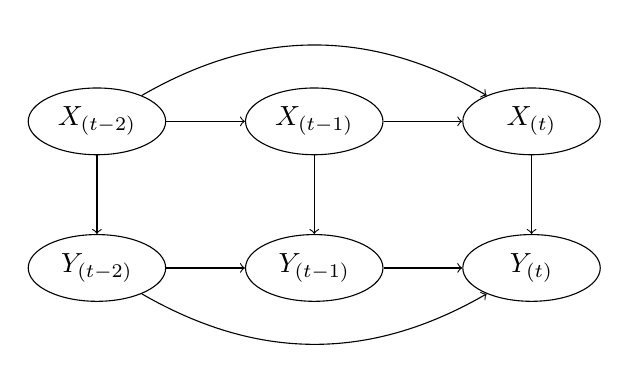
\begin{tikzpicture}[
  node distance=1cm and 1cm,
  mynode/.style={draw,ellipse,text width=1cm,align=center}
]
\node[mynode] (x0) {$X_{(t-2)}$};
\node[mynode,below =of x0] (y0) {$Y_{(t-2)}$};
\node[mynode, right=of x0] (x1) {$X_{(t-1)}$};
\node[mynode,below =of x1] (y1) {$Y_{(t-1)}$};
\node[mynode, right=of x1] (x2) {$X_{(t)}$};
\node[mynode, below=of x2] (y2) {$Y_{(t)}$};

\path[->] (x0) edge (y0);
\path[->] (x1) edge (y1);
\path[->] (x2) edge  (y2);
\path[->] (x0) edge (x1);
\path[->] (x1) edge (x2);
\path[->] (y0) edge (y1);
\path[->]  (y1) edge (y2);
\path[->]  (x0) edge[bend left] (x2);
\path[->]  (y0) edge[bend right] (y2);

\end{tikzpicture}
\caption{Example of a dynamic Bayesian network with Markov order $t=2$.}
\label{fig:dynamicBN}
\end{figure}



\begin{figure}[h]
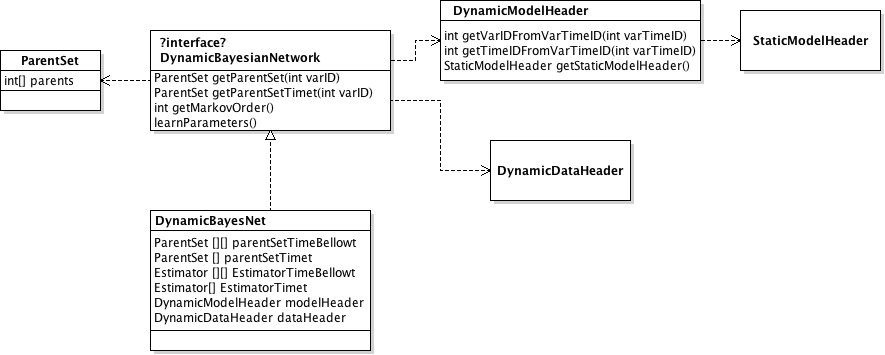
\includegraphics[width=\textwidth]{DynamicBN}
\caption{Class diagram for the dynamic BNs.}
\label{fig:classDiagramDynamicBN}
\end{figure}

Let $X_1,\ldots,X_N$ the set of variables. In order to identity a variable in a time $t$, we use the following indexes:

\begin{itemize}
\item Time $t$: $[0, 1, \ldots, N-1]$
\item Time $t-1$: $[N, 1, \ldots, 2N-1]$
\item Time $t-2$: $[2N, 1, \ldots, 3N-1]$
\end{itemize}

The class diagram of a dynamic model is shown in Fig.~\ref{fig:dynamicBN}. 
To represent the model structure we are going to use 2 attributes: 

\begin{itemize}
\item \texttt{parentsAtTimet}: a vector of ParentSet of size $N$. At each position a vector of indexes (see above) are stored. 
\item \texttt{parentsAtTimeBellowT}: a matrix of ParentSet. The first component is devoted to identify the index of the variable (from 1 to $N$).
The second component identities the time. For the example of order two, the dimension of this second component is 2 ($t-1$ and $t-2$).
\end{itemize}

The same strategy is used to store the attributes \texttt{EstimatorTimet} and \texttt{EstimatorTimeBellowt}.

Similar to the static approach, we will use an interface called 
\texttt{DynamicBayesianNetwork} and our implementation of a dynamic BN
is made through class \texttt{DynamicBayesNet}. 


%%%%%%%%%%%%%%%%%%%%%%%%%%%%%%%%%%%%%%%%%%

\section{Estimators and Potentials}
\label{sec:estimator_potential}

We have considered two possible representations of the quantitative component of the 
variables in the model. The idea is to have, on one hand, \emph{Estimators}, specially 
designed to be updated from sufficient statistics during learning.
On the other hand, it should be convenient to have a lighter data structure, 
\emph{Potential}, with the learning results and specially oriented only to inference. 
In this way, we try to optimize both learning and inference. 

Regarding \emph{Estimators} we only consider non-exponential distribution families as
we are using a sufficient statistic-based learning approach. Fig.~\ref{fig:classDiagramEstimators}
shows the data structure considered. The idea is to have an interface \texttt{Estimator} with a set 
of classes implementing it: \texttt{DiscreteEstimator}, \texttt{GaussianEstimator} and \texttt{MultivariateGaussianEstimator}.
For conditional estimator, we define another interface called \texttt{ConditionalEstimators} extending from \texttt{Estimator}.
The implemented conditional estimators cover all the possible structures involving continuous and discrete variables, i.e., 
\texttt{D\_D\_ConditionalEstimator}, \texttt{C\_D\_ConditionalEstimator}, \texttt{C\_DC\_ConditionalEstimator} and \texttt{C\_C\_ConditionalEstimator}.

Data structure for \emph{Potentials} is shown in Fig.~\ref{fig:classDiagramPotentials}. Class \texttt{Potential} will have 
methods for combining, marginalizing  potentials, ... In contrast to the \emph{Estimators}, this class is designed so that their 
probability distributions are not modified.

\begin{figure}[h]
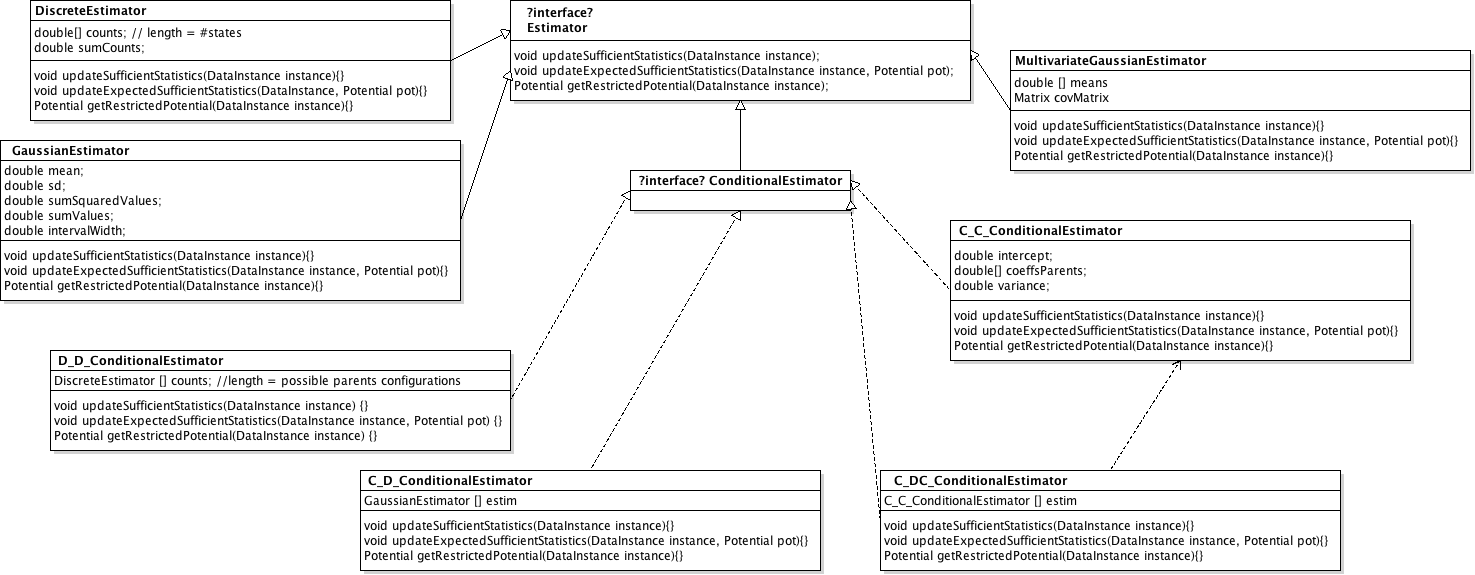
\includegraphics[width=\textwidth]{Estimators}
\caption{Class diagram for the Estimators.}
\label{fig:classDiagramEstimators}
\end{figure}


\begin{figure}[h]
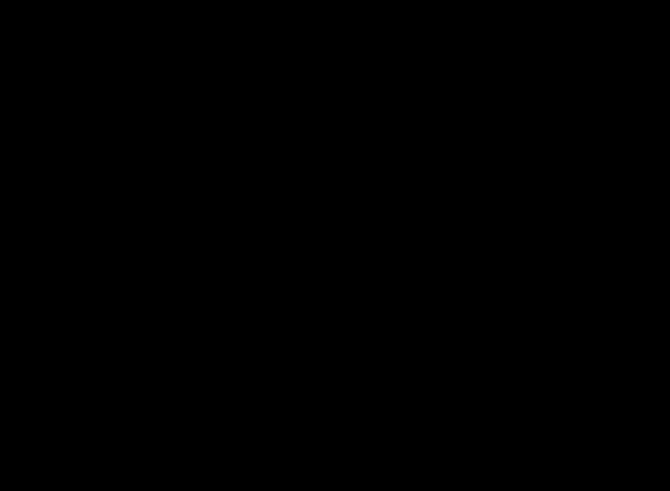
\includegraphics[width=\textwidth]{Potential}
\caption{Class diagram for the Potentials.}
\label{fig:classDiagramPotentials}
\end{figure}


%%%%%%%%%%%%%%%%%%%%%%%%%%%%%%%%%%%%%%%%%%
\section{Database}

For modeling the data structures related to the dataset, there are several issues 
and limitations to be considered. Firstly, data (in general) will not be loaded in memory so streaming
techniques are considered instead. 
Secondly, the data processing for learning dynamic models requires a special treatment (at least in Cajamar).
For the sake of efficiency, we propose to design separately static and 
dynamic representations of the database structure for static and dynamic models, respectively. 
Also, because a same problem rarely implies the use of both representations of the database simultaneously.

Let consider the following notation. 

Variables: $X_1, \ldots, X_n$

A dataset $\cal{D}$ contains a set of elements in the form $\{\x^{(1)}, \x^{(2)},\ldots, \x^{(m)}\}$, 
where each $\x^{(i)}=(x_1^{(i)}, \ldots, x_n^{(i)})$ represents a data instance.





%%%%%%%%%%%%%%%%%%%%%%%%%%%%%%%%%%%%%%%%%%

\subsection{Static Database}
\label{subsec:staticDatabase}

\begin{figure}[h]
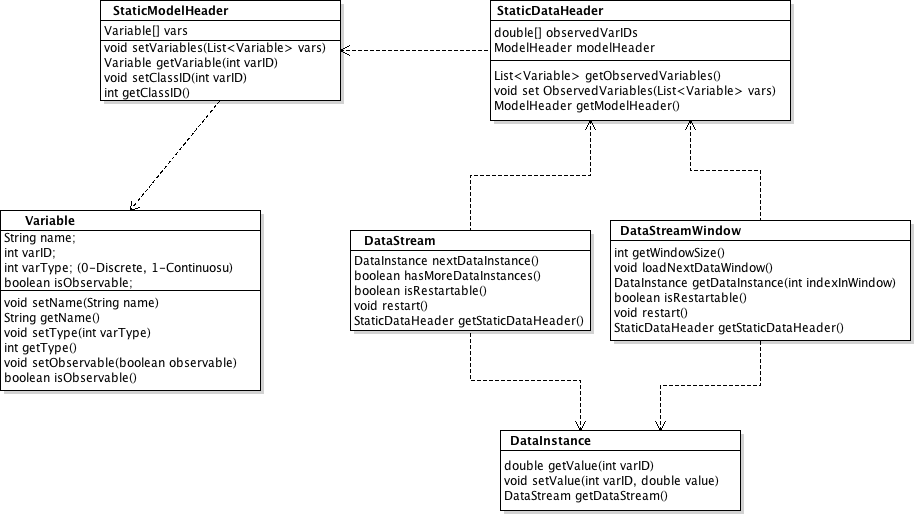
\includegraphics[width=\textwidth]{StaticDB}
\caption{Class diagram for the static database.}
\label{fig:staticDB}
\end{figure}

The static representation of the database shown in  Fig.~\ref{fig:staticDB} will be 
used for learning a static model under data streaming. Class 
\texttt{DataInstance} represents a unique instance $\x^{(i)}$ of the dataset. The idea is to
have an \emph{iterator} class responsible for processing the different data instances 
in the database. This is made by class \texttt{DataStream}. 

In the same level, class \texttt{DataStreamWindow} covers the situation in which 
going back in the set of data instances is somehow required for updating the 
estimators. It represents a memory window with the latest $n$ data instances 
processed so far.

Class \texttt{StaticDataHeader} will store general information about the variables. 
First, a vector indicating which variables are observed and second, the list of variables
with their information (\texttt{class StaticModelHeader}). There is a class \texttt{Variable}
with the attributes \emph{name}, \emph{varID} (useful to identify and process a 
variable efficiently), among others.



\subsection{Dynamic Database}
\label{subsec:dynamicDatabase}
\begin{figure}
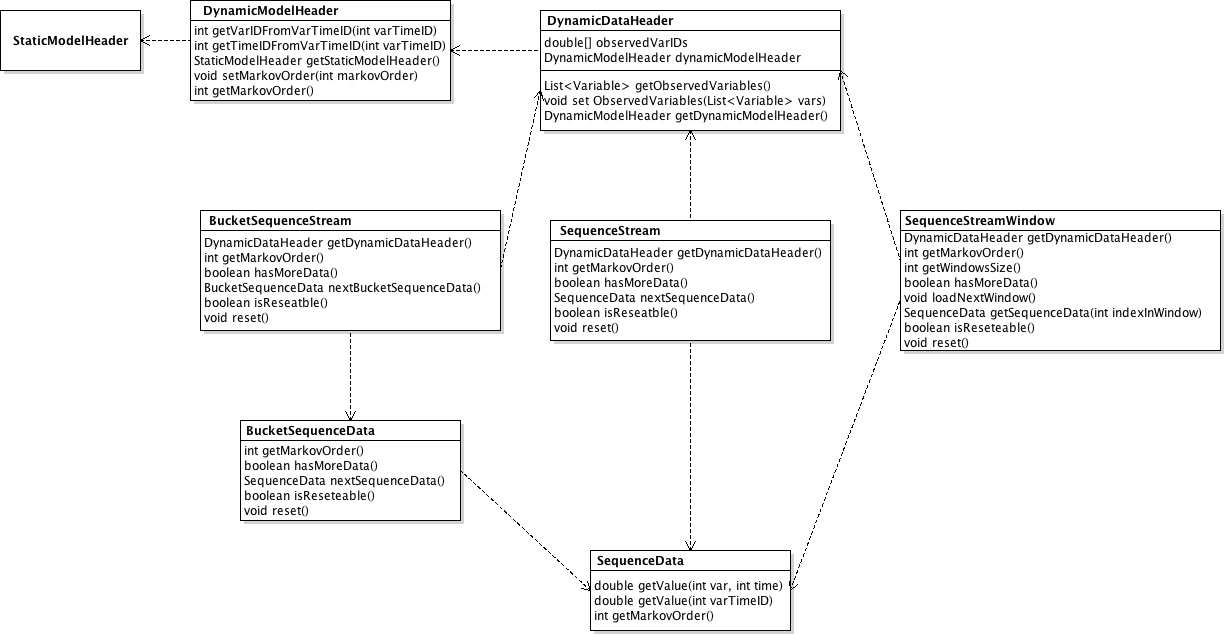
\includegraphics[width=\textwidth]{DynamicDB}
\caption{Class diagram for the dynamic database.}
\label{fig:dynamicDB}
\end{figure}

The dynamic processing of the dataset leads to a more complex design. We have identified two possible ways of arriving streaming data:

\begin{enumerate}
\item Each time $t$ a set of values for the variables arrives. For $t=2$ this will be a \texttt{SequenceData} object:
	\begin{center}
	\begin{tabular}{|c|c|c|}
	\hline
	$\x_{(t-2)}$ & $\x_{(t-1)}$ & $\x_{(t)}$\\
	\hline
	\end{tabular}
	\end{center}
	
	 

\item Each time $t$ a set of values for the variables for a set of individuals arrives. This is the case of Cajamar in which every day we have a data matrix with values for all the variables and all the clients:

	\begin{center}
	\begin{tabular}{|c|c|c|c|}
	\hline
	Client 1  & $\x^{(1)}_{(t-2)}$ & $\x^{(1)}_{(t-1)}$ & $\x^{(1)}_{(t)}$\\
	\ldots      & \ldots  & \ldots  & \ldots \\
	Client m  & $\x^{(m)}_{(t-2)}$ & $\x^{(m)}_{(t-1)}$ & $\x^{(m)}_{(t)}$\\	\hline
	\end{tabular}
	\end{center}
	The idea is that every time we have to process a data matrix (\texttt{BucketSequenceData}) with $m$ rows (each row corresponds to a \texttt{SequenceData} object) and $t$ columns.
\end{enumerate}

\section{Open issues}

\begin{itemize}
\item Consider the situation in which data stream exceeds the data processing of the system. A kind of buffer could be a solution. 
\item Scalability inside the algorithms. Does it influence the definition of the prototype or only when including the learning/inference algorithms?
\item Buy some licenses of IntelliJ to work with UML diagrams linked to the code. 
\end{itemize}

 


\end{document}          
